\chapter{开集识别}

\section{YOLOOC：开集物体检测与新类别发现}

\begin{figure}[H]\centering
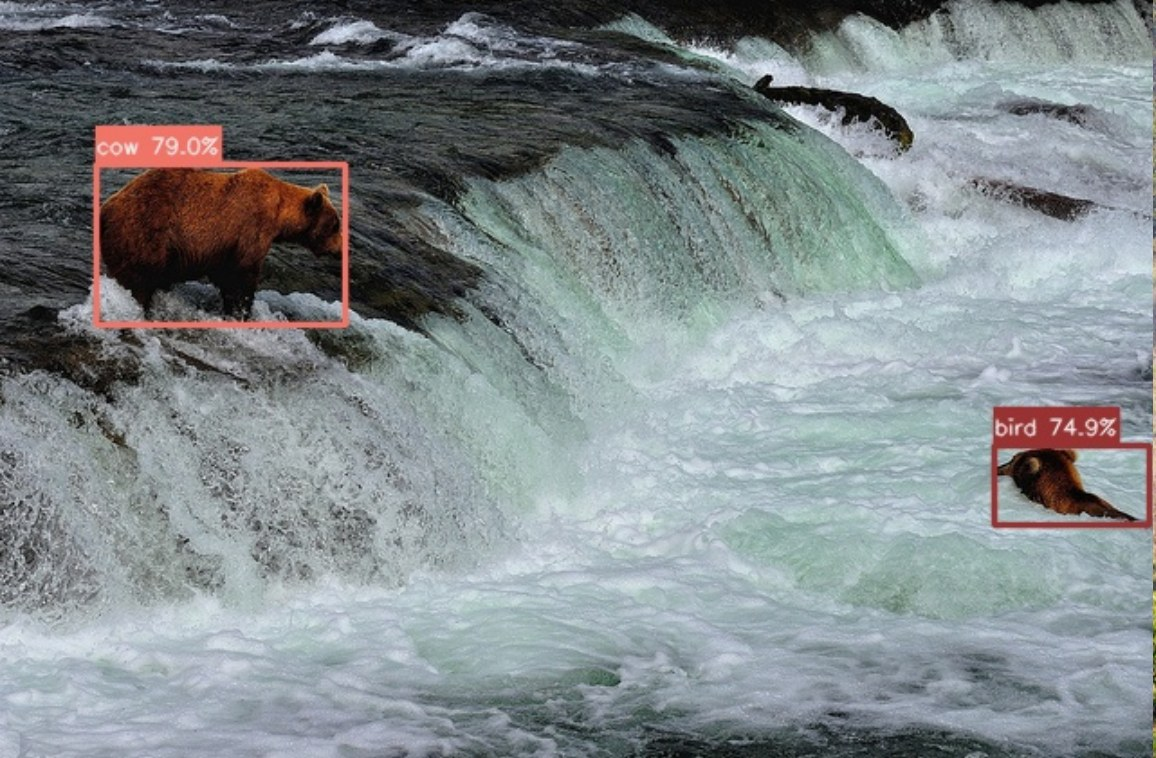
\includegraphics[width=0.82\linewidth,height=0.42\textheight,keepaspectratio]{figures/bear.jpg}
\end{figure}

在《DML：为什么模型的置信度不等于模型对世界的认识程度？》《DPM：视觉语言模型如何认识未知？——从语义识别到分布认知》《ASL：既然方向很重要，能不能在训练阶段塑造更好的角度空间？》《OSPCoOp: 从识别未知类别，到识别模型判断中的错误依据》系列中，我们系统思考了 AI 模型（比如 Transformer、CLIP）如何发现训练分布之外的数据，或者说检测数据分布的偏移。无论是基于分类置信度、特征距离，还是视觉语言模型中的语义匹配，核心问题都是：当一个测试样本到来时，模型能否判断它是否属于训练时已知的数据分布？但当我们把这一问题从图像分类扩展到物体检测时，情况就变得复杂了。一张图像中可能包含多个物体，其中既有模型训练时见过的类别，也可能出现从未见过的物体。传统物体检测模型在训练时，通常只学习预先定义好的类别。比如训练集有 20 种类别，那么模型就围绕这 20 种类别学习物体定位和分类。当它遇到第 21 种类别时，会出现一个问题：它可能把这个新物体错误地识别成已有类别，也可能直接忽略它。我们不能简单地将整张图像判定为分布内或分布外，而是需要进一步回答：图像中有哪些物体？它们分别位于什么位置？哪些属于已知类别？哪些是模型尚未认识的未知物体？这意味着，开放世界场景下的物体检测不仅需要完成传统的物体定位与分类，还需要具备识别未知实例的能力。模型不能因为一个物体不属于已有类别，就将其直接忽略，或者错误地归入某个已知类别。因此，开放集物体检测首先要解决的是：如何让模型在没有见过某个类别的情况下，仍然能够发现这个物体？

第一步：让模型找到未知物体，而不是只把它们当成背景

\begin{figure}[H]\centering
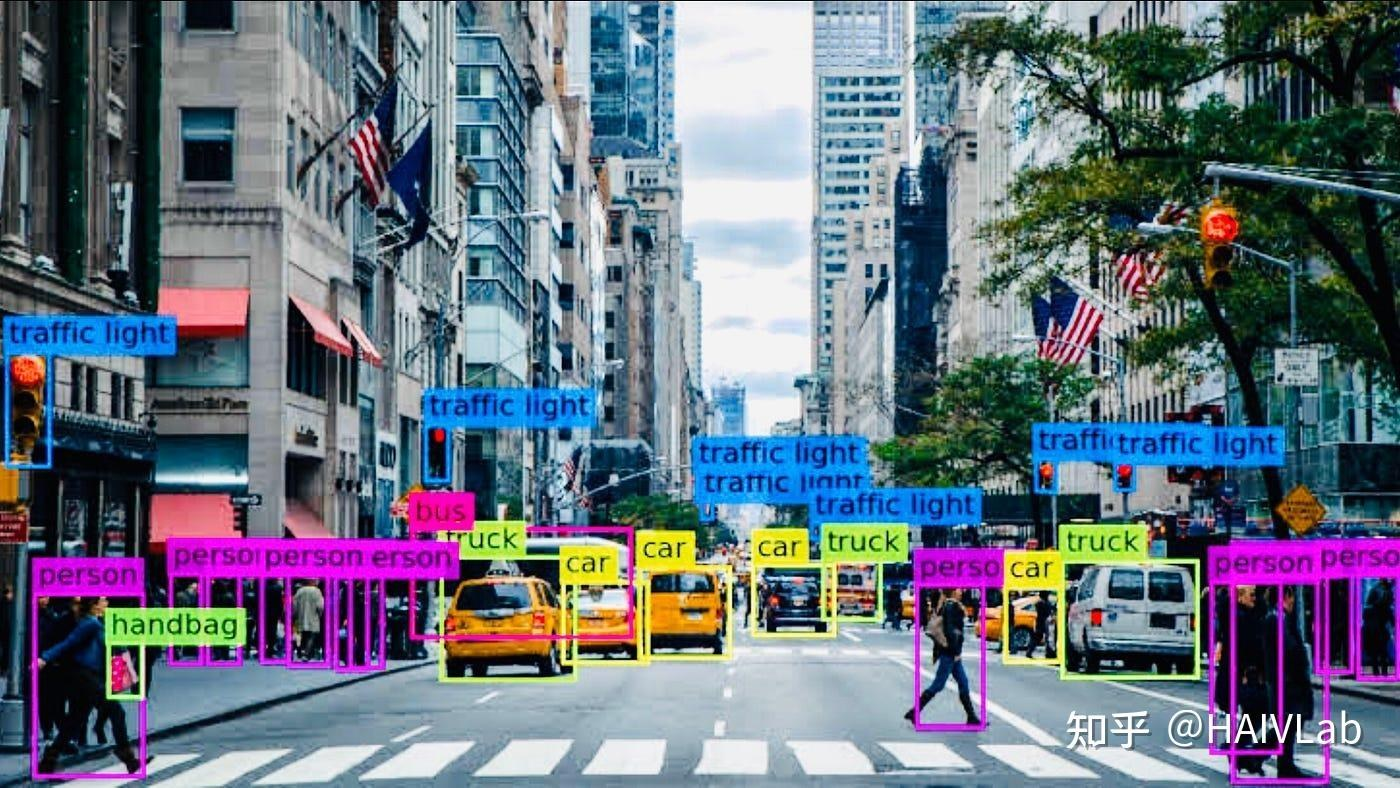
\includegraphics[width=0.82\linewidth,height=0.42\textheight,keepaspectratio]{figures/city.jpg}
\caption*{以类别无关物体定位（Class-Agnostic Localization）为基础}
\end{figure}

训练定位模块时，不再使用常规的类别分类损失，而主要优化两个目标：

\begin{itemize}
  \item Bounding Box Loss：让预测框尽可能准确地包围物体。
  \item Objectness Loss：判断一个区域是否存在物体。
\end{itemize}

分类监督会引导模型学习已知类别的特征。如果模型在训练过程中始终被要求把物体归入已有类别，就可能形成对已知类别的偏向，进而影响它对未知物体的泛化能力。所以，这里的基本思想是：先学习什么是一个物体，再学习这个物体是什么。定位之后，还需要对物体进行语义理解。为此，可以引入 CLIP 这样的视觉语言模型。具体来说，将检测到的候选区域输入图像编码器，将类别描述输入文本编码器，然后比较两者在共同语义空间中的余弦相似度。通过调整文本提示中的上下文向量，可以进一步适应当前的检测任务。第二步：从未知实例中发现新类别

假设模型已经能够在图像中找到未知物体。现在，它连续看到十个未知物体。它们可能分别是三辆叉车、四辆清扫车和三辆工程车。如果模型把它们全部标记成 Unknown，虽然完成了未知检测，但并没有真正理解这些物体。我们希望模型进一步发现：这十个未知实例可能包含三个不同的新类别。这就涉及 Novel Class Discovery（新类别发现）。它和前面的未知检测有一个重要区别：

\begin{itemize}
  \item 未知检测：判断一个物体是不是已知类别。
  \item 新类别发现：进一步分析未知物体之间的关系，找出潜在的新类别。
\end{itemize}

一个基本思路是利用物体的特征表示。如果两个未知物体在视觉特征空间中比较接近，那么它们可能属于同一个类别；如果它们之间存在明显差异，就可能属于不同类别。通过对未知物体进行特征分析和聚类，模型可以将原来统一的 Unknown 拆分成多个潜在类别。但这里有一个实际困难：传统的新类别发现方法，往往需要提前提供一些新类别数据，哪怕只是弱标注，也意味着我们已经知道新类一个更严格的开放类别设定是：新类别在训练阶段完全不可见，只能在模型实际运行时出现。在这样的设定下，YOLOOC 使用 YOLO 架构构建开放类别物体检测器，并引入 Label Smoothing 来缓解模型对已知类别的过度自信。别可能出现。普通分类训练通常使用 One-Hot Label。例如，一张汽车图片对应的标签可以表示为：

\[
[1,0,0,0]
\]

模型被要求把汽车类别的概率推到 1，其他类别推到 0。但是，如果模型遇到一辆从未见过的特殊车辆，它仍然可能被迫在已有类别中作出选择。Label Smoothing 则将原本非常确定的标签适当软化，例如：

\[
[1,0,0,0]\;\rightarrow\;[0.9,\,0.033,\,0.033,\,0.033]
\]

这使模型不必把所有非目标类别的响应都压到绝对的零，也有助于缓解模型对已知类别的过度自信。在 YOLOOC 的开放类别设置中，这种处理被用于帮助模型避免把新类别过早、过于自信地归入已有类别，从而为新类别发现创造条件。Label Smoothing 本身并不等于聚类，也不会自动给未知物体命名。它主要是在训练阶段调整模型的分类行为，让模型在面对新类别时保留一定的识别空间。新类别发现仍然是一个需要进一步解决的问题。YOLOOC 这一工作的关键推进在于：不再仅仅把未知物体当成需要拒绝的对象，而是开始考虑如何从未知物体中发现新的类别，并为后续增量学习做准备。

\subsubsection*{第三步：模型运行过程中动态调整自己的判断}

前面两步关注的是如何发现未知物体，以及如何从未知物体中发现新类别。但还有一个问题：模型在部署之后，能不能随着新物体的出现，及时调整自己的判断方式？假设一个模型最初只认识汽车、卡车和行人。部署一段时间后，它遇到了一辆新型工程车辆。由于分类器是在原有类别上训练出来的，它可能会把工程车辆错误地判断为卡车。这里的问题不一定是模型完全没有提取到工程车辆的特征，而是分类器的权重和决策边界已经形成了对已知类别的偏向。

可以把分类器理解为一个裁判。训练完成后，这个裁判已经形成了一套固定的判断标准。无论外面出现什么新物体，它都倾向于用原来的标准进行分类。那么，能不能让这个裁判在实际运行过程中，适当调整自己的判断标准？这就是动态权重校准（Dynamic Weight Calibration）的基本思想。Stay Open 关注的是模型在推理阶段遇到新类别时的开放世界检测问题。它将 Label Smoothing 引入模型的分类行为，并利用已知类别与新类别对标签平滑的不同响应，帮助模型区分已知物体与新出现的物体。可以用一个简单的例子理解：

\begin{itemize}
  \item 对于模型已经充分学习过的汽车，它的类别判断通常比较稳定；
  \item 对于模型从未见过的新型车辆，分类响应可能对标签平滑更加敏感；
  \item 这种响应差异可以作为判断物体是否属于新类别的线索。
\end{itemize}

因此，关键不只是把标签变软，而是利用模型对标签平滑的响应变化，校准分类器对已知和未知物体的判断。

总而言之，这一系列工作延续了前面 OOD Detection 的基本思想，但研究对象和目标已经发生了变化：我们不再只问模型能否判断一个样本是否来自已知分布，而是进一步追问，模型能否在复杂场景中找到未知物体、发现未知类别，并逐步适应不断变化的开放世界。相关工作：

\begin{itemize}
  \item Qinhao Zhou, Xiang Xiang. Stay Open: Calibrating Weights Continuously for DetectingOutof-DistributionObjects on the Fly. In PRCV, 2024.
  \item Q Wan, X Xiang*, Q Zhou. YOLOOC: YOLO-based Open-Class Incremental Object Detection
\end{itemize}

withNovel Class Discovery. ArXiv preprint: 2404.00257, 2024.

\begin{itemize}
  \item •
\end{itemize}

Q Wan, S Wang, X Xiang*. A Simple Unknown-Instance-Aware Framework forOpenSetObject Detection. In ICIST, 2023. Xiang Xiang*, Qinhao Zhou, Zhuo Xu, Jing Ma, Jiaxin Dai, Yifan Liang, Hanlin Li. OpenHAIV: A Framework Towards PracticalOpen-WorldLearning. ArXiv preprint: 2508.07270, 2025.

\section{MCAS：基于层次化属性的开放集识别与理解}

在《YOLOOC：开集物体检测与新类别发现》中，我们逐渐解决了几个问题：如何找到未知目标，如何从未知实例中发现潜在的新类别，以及如何调整模型的判断机制，使其能够更好地应对训练阶段没有见过的类别。但这里还有一个值得进一步思考的问题：当模型遇到一个未知类别时，它究竟能够理解多少？

传统的开放集识别（Open-Set Recognition）通常采用一种相对直接的处理方式：模型先对输入样本进行分类，如果它与所有已知类别的匹配程度都不够高，就将其判定为未知类别。例如，一个只学习过猫、狗、马和牛的模型，遇到一只袋鼠时，理想情况下应该拒绝将它归入这四个已知类别，而是输出 Unknown。这当然是必要的。但从人的认知过程来看，这样的结果还不够。即使我们没有见过袋鼠，也可能知道它是一种动物，有四肢、有尾巴，具有某些与其他哺乳动物相似的特征。虽然我们不能准确说出它的具体类别，但仍然能够根据已有知识，对它形成一定程度的理解。换句话说，不知道一个对象的具体类别，并不意味着对它一无所知。这启发我们重新思考开放集识别：能不能让模型在拒绝错误分类的同时，进一步描述未知目标具有哪些属性，以及它可能属于哪个更大的语义类别？为什么需要属性表示？

传统分类模型通常直接建立图像特征与类别标签之间的映射。例如：

\begin{itemize}
  \item 输入一张猫的图片，输出 Cat；
  \item 输入一张狗的图片，输出 Dog；
  \item 输入一张马的图片，输出 Horse。
\end{itemize}

这种方式非常直接，但类别标签本身包含的信息有限。模型知道一个目标是猫，却不一定能够清楚表达它为什么是猫，以及它与其他类别之间有哪些共同特征。属性（Attribute）提供了一种更细致的表示方式。例如，我们可以从以下几个维度描述动物：

\begin{itemize}
  \item 身体是否覆盖毛发；
  \item 是否具有四条腿；
  \item 是否具有长尾巴；
  \item 是否具有翅膀；
  \item 是否具有长脖子；
  \item 是否具有特定的身体形态。
\end{itemize}

\begin{figure}[H]\centering
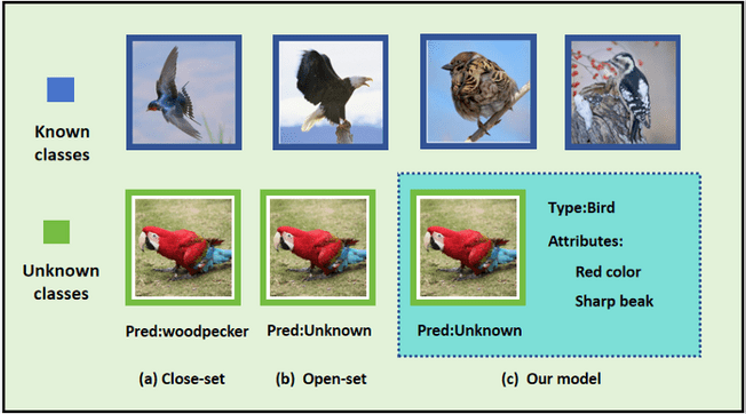
\includegraphics[width=0.82\linewidth,height=0.42\textheight,keepaspectratio]{figures/mcas_birds.png}
\caption*{不仅能够将未见过的目标识别为未知类别，还能提供其所属的粗粒度类别及相关属性信息}
\end{figure}

这样，一个类别就不再只是一个孤立的标签，而是由一组属性共同描述。例如，猫和狗都具有毛发、四肢等属性，但在身体形态、耳朵、尾巴等方面又存在差异。袋鼠虽然不是训练时见过的类别，但它仍然具有一些与已知动物共享的属性。因此，属性可以成为连接不同类别的一种中间表示。我们不再仅仅学习：$\text{Image}\rightarrow\text{Category}$。而是进一步学习 $\text{Image}\rightarrow\text{Attributes}\rightarrow\text{Category}$。这里的关键变化是：模型不再只依赖类别标签，而是同时学习图像与属性之间的关系。属性具有一定的语义含义，而且往往能够跨越具体类别共享。对于开放集识别而言，这种共享性尤其重要：即使一个类别没有出现在训练集中，它仍然可能具有模型已经学过的某些属性。

从属性表示到层次化属性空间

不过，仅仅引入属性还不够。假设我们有一组动物类别，每个类别都对应一组属性。我们可能会发现，某些属性在很多类别之间重复出现，而另一些属性则更有区分能力。例如：

\begin{itemize}
  \item “具有四肢”“具有毛发”可以帮助描述一个较宽泛的动物范围；
  \item “具有长脖子”“具有明显的斑点”则可能更有助于区分某些具体类别。
\end{itemize}

前一类属性更偏向粗粒度语义，后一类属性则更偏向细粒度语义。这就引出了一个重要问题：能不能利用类别之间的层次关系，把属性空间进一步分解？

在 Maximum Category-Attribute Score（MCAS）这项工作里，采用的基本思路是：先根据类别属性之间的相似性，将已知类别划分为若干个较大的类别组，再分析每个类别组内部共享哪些属性。具体来说，可以分成两个步骤。第一步：根据属性相似性组织类别。每个类别都对应一个属性原型（Attribute Prototype），可以理解为描述这个类别的一组属性向量。例如，如果两个类别具有大量相似的属性，那么它们的属性原型在特征空间中就会比较接近。通过对类别属性原型进行 K-means 聚类，可以把相似的类别组织到同一个粗粒度类别组中。第二步：把共享属性和区分属性分开。在每个类别组内部，统计不同属性在组内类别中的出现频率。如果某个属性在组内大多数类别中都出现，那么它更适合作为描述这个大类的粗粒度属性；如果它只出现在部分具体类别中，则可以作为进一步区分类别的细粒度属性。例如，在一个假设的动物类别组中：共同具有的毛发、四肢等属性，可以描述较宽泛的类别范围；不同动物特有的身体形态、耳朵和尾部特征，则可以帮助区分组内的具体类别。这样，每个类别的属性表示就可以拆分成两部分：$A_i=A_i^{c}+A_i^{f}$。其中，$A_i^{c}$ 表示粗粒度属性，$A_i^{f}$ 表示细粒度属性。这里的加法主要用于直观理解：原来的属性集合被分成了共享部分和更具区分性的部分。实际方法通过属性掩码来移除粗粒度属性，得到细粒度属性原型。

\begin{figure}[H]\centering
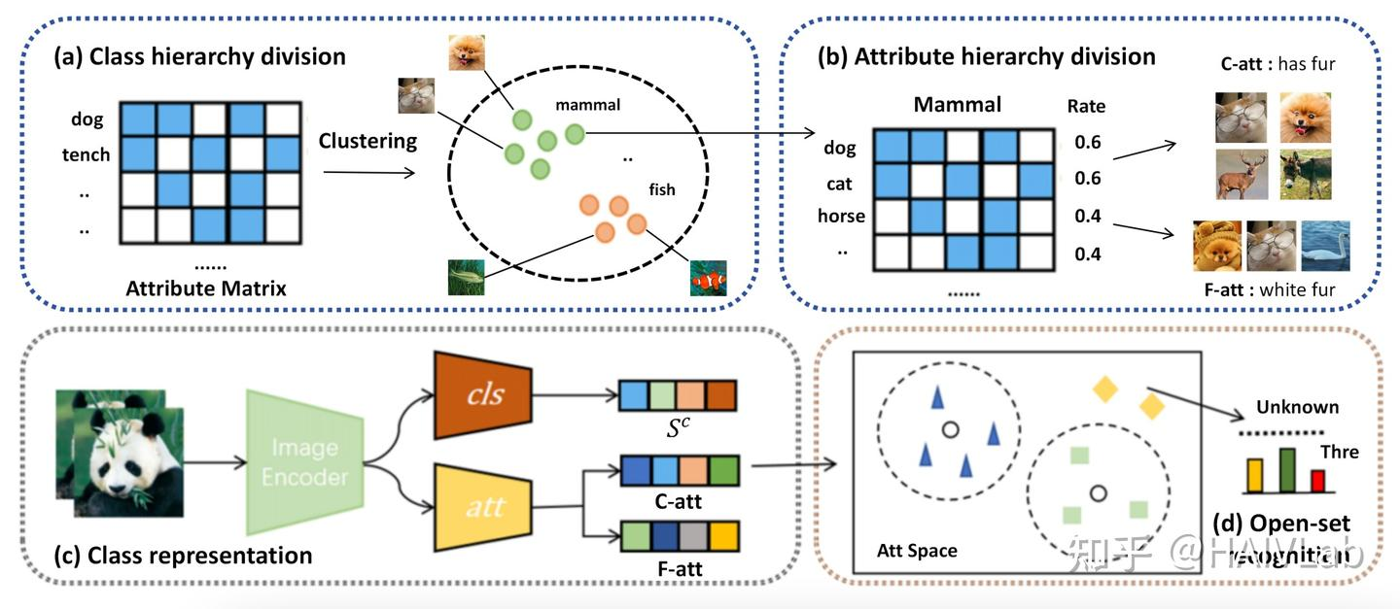
\includegraphics[width=0.82\linewidth,height=0.42\textheight,keepaspectratio]{figures/mcas_hier.png}
\caption*{首先为每个类别建立层次结构，进而构建属性层次结构，将属性空间划分为多个细粒度属性空间；再通过利用属性信息和类别标签进行监督学习，最终在细粒度属性空间中完成开放集识别}
\end{figure}

如果只在完整属性空间中比较两个类别，那么大量共享属性可能会掩盖它们之间真正重要的差异。将粗粒度属性分离之后，我们就可以在相应的类别组内部，重点比较更有区分能力的细粒度属性。因此，这种层次化设计并不是简单地增加属性数量，而是希望根据类别之间的关系，让属性表示更加有针对性。

如何让图像进入属性空间？

有了类别属性原型，下一步就是让模型能够从图像中预测属性。这项工作采用一个双分支结构，共享同一个视觉特征提取网络，但分别承担类别预测和属性预测两个任务。给定一张输入图片，首先通过视觉骨干网络提取特征：

\[
F_v=\Phi_F(x)
\]

然后分别送入两个分支：

\[
\begin{gathered}\hat{A}=\Phi_A(F_v) \\ p^{c}=\Phi_C(F_v)\end{gathered}
\]

其中 $\hat{A}$ 是模型预测的属性向量；$p^{c}$ 是模型对已知类别的预测概率。可以把这两个分支理解为两个相互配合的观察角度：一个回答“它是什么类别”，另一个回答“它具有哪些属性”。训练时，类别分支使用交叉熵损失，属性分支使用二元交叉熵损失。两者共同优化：$\mathcal{L}=\mathcal{L}_C+\lambda\mathcal{L}_A$。这样，模型在学习类别区分能力的同时，也需要学习更加细致的视觉语义属性（对于缺少属性标注的数据集，这项工作利用 Qwen-VL-Chat 为类别生成文本描述，再对这些描述进行聚类，整理出类别对应的二值属性矩阵。对于已有属性标注的数据集，也使用相应的属性信息构建属性表示）。

遇到未知类别时，如何利用属性进行判断？

前面解决了如何学习类别和属性表示。真正关键的是：当测试阶段出现一个未知类别时，属性究竟如何帮助模型？假设模型已经学习过猫、狗、马等类别，现在遇到一张从未见过的动物图片。传统开放集识别主要依据分类分数判断它是否属于已知类别。如果所有已知类别的匹配分数都不够高，就将它判定为未知。但在 MCAS 这项工作中，还可以多利用一层信息：即使具体类别判断不可靠，属性预测仍然可能提供有价值的线索。具体做法是结合类别分支和属性分支的结果——首先，类别分支给出最可能的已知类别。根据这个类别，模型确定它所属的粗粒度类别组；然后，模型根据该类别组对应的属性掩码，提取测试样本的细粒度属性表示；接下来，将这个预测属性向量与该类别组中各个已知类别的细粒度属性原型进行比较，计算余弦相似度。这样，就得到两种判断依据：类别分数——当前图像与已知类别的直接匹配程度；属性分数——当前图像预测出的属性，与候选类别属性原型的相似程度。最后，将两者 结合：$S^{ca}=S^{c}+\beta S^{a}$。 最终的最大类别—属性分数即称为 MCAS（Maximum Category-Attribute Score）。如果 MCAS 高于设定阈值，模型就认为该样本可以归入某个已知类别；如果低于阈值，则判定为未知类别。这里的关键不在于简单地增加一个属性分类器，而在于让类别判断和属性判断相互补充。一个未知类别可能与某个已知类别在整体外观上比较接近，但在细粒度属性上存在明显差异。此时，属性分支可以提供额外的判断依据，帮助模型降低对错误已知类别的置信度。更重要的是，模型还能够输出属性预测结果，以及对应的粗粒度类别信息。例如，它可能无法判断一只动物究竟属于哪一种具体物种，但可以提供它具有哪些属性、与哪个较大的类别组更接近等信息。这就使得开放集识别的输出不再只是一个 Unknown 标签，而是包含了更多可供人理解的信息。实验方面，这项工作在两类数据设置上进行了评估。第一类是细粒度语义变化场景，包括CUB-200-2011 鸟类数据集、Stanford Cars 汽车数据集和 FGVC-Aircraft 飞机数据集。第二类是具有属性标注的数据集，包括 AWA2 和 LAD。实验主要使用 AUROC 和 OSCR 等开放集识别指标，评价模型区分已知与未知样本的能力。结果表明，结合类别监督和属性监督，并进一步利用层次化属性空间，可以在这些开放集识别任务中取得较好的表现。其中有几个值得关注的发现：

\begin{itemize}
  \item 单独使用类别信息或属性信息，都不如将两者结合起来。
  \item 类别与属性的联合学习能够让视觉特征同时包含类别判别信息和属性语义信息。
  \item 对属性空间进行层次化分解，能够进一步改善细粒度开放集识别效果。
  \item 属性空间并不是越大越好，属性数量和筛选方式也会影响最终表现。
\end{itemize}

这说明，属性信息的价值并不只是让模型给出更容易理解的描述。经过合理组织之后，它还能够为开放集识别提供额外的判别依据。

总而言之，在更大的研究脉络中，结合前面的开集物体检测研究，我们认识到：模型面对未知目标时，不能只给出一个 Unknown 标签，而应该尽可能发现未知目标之间的关系，甚至进一步发现新的类别。MCAS 这项工作则从另一个角度推进了这个问题。它没有直接要求模型完成新类别聚类，也没有要求模型将新类别增量地加入分类器，而是尝试利用类别属性和层次化语义关系，让模型对未知类别形成更细致的认识。这实际上引入了一种新的思考方式：已知类别之间并不是相互孤立的，它们共享属性、具有层次关系；未知类别也可能与已有类别共享部分属性。如果我们能够学习和利用这些关系，那么模型就不必把已知和未知看成完全割裂的两部分。这也为后续的持续学习研究提供了一个自然的出发点——从开放集识别走向持续学习是一个重要的过渡。模型需要学习的不只是孤立的类别标签，还包括类别之间的结构关系，以及这些关系在新知识到来时如何变化。从这个角度看，层次化属性空间提供了一种有意义的语义组织方式：它让我们从类别标签进一步走向属性和类别结构，从而为后续研究类别增量、语义细化和持续学习提供了思路。开放集识别回答的是：面对未知类别，模型能否识别它不是已知类别？而持续学习进一步追问：当这些未知类别逐渐变成需要学习的新类别时，模型如何吸收它们，同时保持已有知识？这两个问题连接起来，才构成了从开放集识别走向开放世界持续学习的一条完整研究路线。相关工作：

\begin{itemize}
  \item Zhuo Xu, Xiang Xiang. Learning Visual-Semantic Hierarchical Attribute Space for
\end{itemize}

InterpretableOpen-Set Recognition. In WACV, 2025.
